\chapter{Diseño Firmware}
\label{diseño_firmware}


\paragraph{} El firmware se ha desarrollado acordemente con el microcontrolador seleccionado, el \textit{ESP8266EX en formato 12F}. Para ello, se ha realizado uso de la ficha técnica del procesador de \textit{expressif} \cite{esp-datasheet} y de la ficha técnica de la pantalla seleccionada \textit{waveshare} \cite{waveshare-datasheet}.

\section{La pantalla}

\paragraph{} Para la pantalla, desafortunadamente, el fabricante no proporciona una librería para el microcontrolador escogido, pero implementar una no es complicado. El dispositivo consta con una interfaz de comunicación \textit{SPI} \cite{motorola-spi} tal y como se muestran en la figura \ref{fig:tfg:04:waveshare_arduino_library_capture_spi}, cuyos comandos están definidos en el datasheet \cite{waveshare-datasheet}.

\paragraph{} Aun teniendo los documentos donde se detalla el funcionamiento de ambos componentes, durante las pruebas de integración, se experimentó un problema con la ventana de tiempo de reinicio de la pantalla de tinta electrónica, dicha ventana de tiempo no consta en el manual, y el uso de ingeniería reversa fue necesaria.

\paragraph{} Dicha ingeniería reversa fue realizada empleando el uso de el analizador de señales \textit{hantek 4032L} y el osciloscopio \textit{Rigol DS1102}. Se adjuntan a este documento las capturas realizadas mediante \textit{pulseview} \cite{pulseview}.

\begin{figure}[!htb]
    \centering
    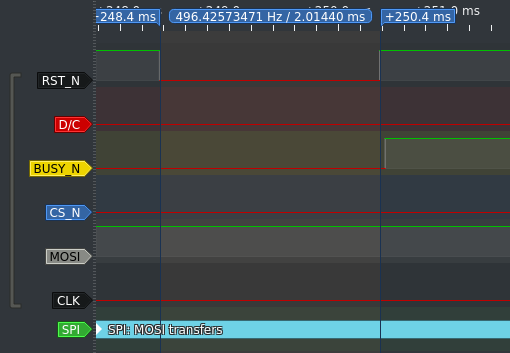
\includegraphics[width=.475\textwidth]{tfg/figuras/04_diseño_firmware/arduino_restart_cap.png}
    \caption{Captura de la señal de reinicio de la librería proporcionada por waveshare para la pantalla}
    \label{fig:tfg:04:waveshare_arduino_library_capture_restart}
\end{figure}

\paragraph{} Tal y como se muestran en la captura y en la figura \ref{fig:tfg:04:waveshare_arduino_library_capture_restart}, dicho tiempo de reinicio era, en la librería aportada por el fabricante de 2 milisegundos.

\begin{figure}[!htb]
    \centering
    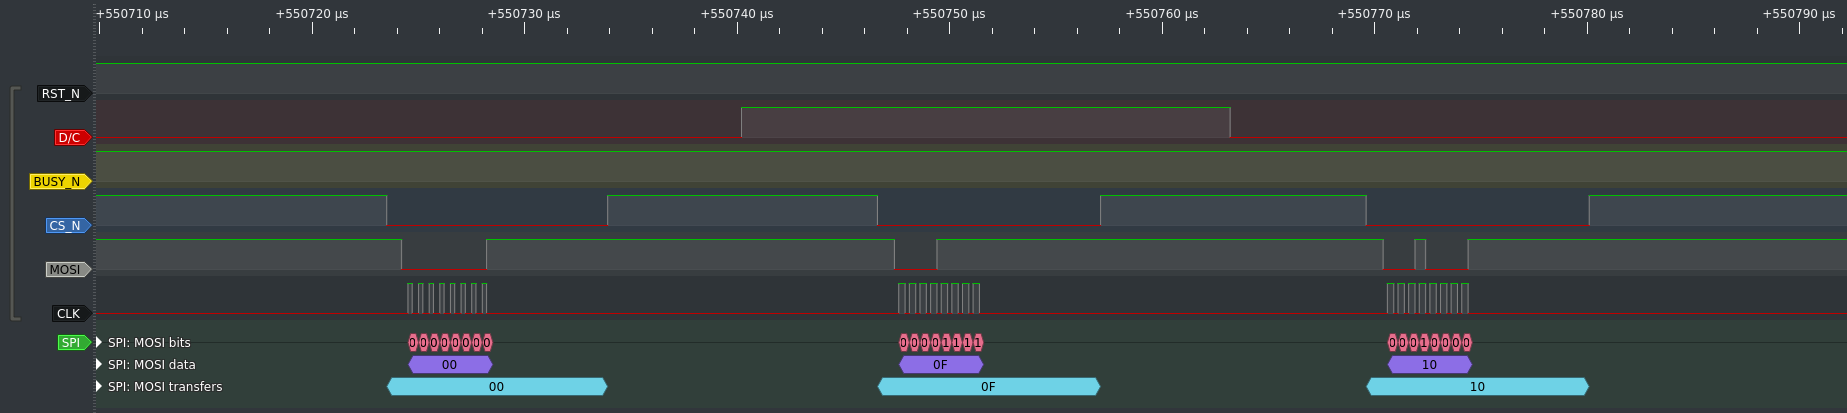
\includegraphics[width=1\textwidth]{tfg/figuras/04_diseño_firmware/arduino_spi_cap.png}
    \caption{Captura de señales spi de la librería proporcionada por waveshare para la pantalla}
    \label{fig:tfg:04:waveshare_arduino_library_capture_spi}
\end{figure}

\paragraph{} Esta demora de 2 milisegundos es un tanto complicada en el \textit{ESP8266EX}, puesto que el tiempo de tick de este microcontrolador es de 10 milisegundos, pero realizando NOP's \cite[página 52]{xtensa-isa} se puede conseguir cualquier tiempo deseado.

\paragraph{} En la ficha técnica de la pantalla también podemos observar que una trama spi de 9 bits ha de ser empleada para comunicarse con el dispositivo, sin embargo, tal y como se puede observar en la figura \ref{fig:tfg:04:waveshare_ardduino_library_capture_spi}, la trama es de 8 bits en la librería proporcionada por el fabricante, y aunque realizando uso de tramas de 9 bits el funcionamiento es correcto, se emplearán tramas de 8 bits para la librería codificada.

\subsection{Nivel de framebuffer}

\paragraph{} Para poder modificar la imagen mostrada en pantalla, disponemos de dos comandos de transmisión de datos, uno para cada color con el que la pantalla puede emplear. Una vez enviemos dicho comando, procederemos a transmitir en tramas de 8 bits los valores de cada pixel con cada bit de dichas tramas, este proceso se repetirá hasta que todos los pixeles de la pantalla hayan recibido un nuevo valor (300x400 pixeles).

\paragraph{} También existe la posibilidad de enviar solo a una región de interés o \textit{ROI} del ingles Region Of Interest mediante un comando para cada color.

\paragraph{} Una vez tenemos cargados en la memoria de la pantalla la imagen que deseamos mostrar, podemos proceder a enviar el comando de actualización de pantalla, el cual refrescará la pantalla con los nuevos datos en su memoria \textit{framebuffer}.

\subsection{El pintor}

\paragraph{} Para abstraernos de realizar las operaciones de escritura a nivel de \textit{framebuffer} se agregará una capa de \textit{pintor}, la cual será encargada de la tarea de acceder y modificar a dicha memoria para pintar objetos y formas más elaboradas que pixeles, como pueden ser rectángulos, círculos o letras.

\paragraph{} Este pintor se puede completar con funciones como pintar una cadena de texto, dibujar un titulo para la pantalla, lista de elementos o pintar una imagen.

\section{Comunicaciones con el servidor central}

\paragraph{} Adicionalmente, una interfaz de comunicación con el servidor central ha de ser codificada, está ha de ser capaz de identificarse y acreditar su identidad ante el servidor, el cual proveerá la información requerida por el mismo, siendo dicha información textos e imágenes dependiendo lo configurado en el servidor central para esa determinada franja horaria y pagina seleccionada por el alumno en el dispositivo físico.


\section{Sensorica}

\paragraph{} Para controlar dicha página, un controlador de sensores capacitivos ha de ser codificado junto a un sistema controlador de la interfaz y comunicaciones para arbitrar todo el sistema.